%----------------------------------------------------------------------------------------
%    PACKAGES AND THEMES
%----------------------------------------------------------------------------------------

\documentclass[aspectratio=169,xcolor=dvipsnames]{beamer}
\usetheme{SimpleDarkBlue}

\usepackage{hyperref}
\usepackage{graphicx} % Allows including images
\usepackage{booktabs} % Allows the use of \toprule, \midrule and \bottomrule in tables
\usepackage{tikz} % For diagrams
\usepackage{fontawesome} % For icons

% Simple boxed placeholder macro for figures (no external files required)
\newcommand{\imgph}[2]{\fbox{\parbox[c][#2][c]{#1}{\centering \small Image Placeholder}}}

%----------------------------------------------------------------------------------------
%    TITLE PAGE
%----------------------------------------------------------------------------------------

\title{Interactive Multimodal GPT for Tactile--Vision Reasoning}
\subtitle{Graduation Project Presentation}

\author{Haowei Gao}

\institute
{
    Department of Bioengineering \\
    Supervisor: Dr. [Supervisor Name]
}
\date{July 2025}

%----------------------------------------------------------------------------------------
%    PRESENTATION SLIDES
%----------------------------------------------------------------------------------------

\begin{document}

\begin{frame}
    % Print the title page as the first slide
    \titlepage
\end{frame}

\begin{frame}{Overview}
    \tableofcontents
\end{frame}

%------------------------------------------------
\section{Introduction}
%------------------------------------------------

\begin{frame}{Motivation}
    \begin{itemize}
        \item \textbf{Goal}: Infer human-perceived touch attributes (e.g., rough, glossy, elastic) from \textit{RGB photographs} and \textit{tactile sensor visualizations}.
        \item \textbf{Challenge}: Bridging visual appearance and haptic qualities requires multimodal reasoning and careful prompt design.
        \item \textbf{Impact}: Enables material understanding for robotics, assistive tech, and interactive design.
    \end{itemize}
\end{frame}

\begin{frame}{Objectives and Hypothesis}
    \textbf{Hypothesis}: Combining tactile visualizations with photographs and standardized prompts improves tactile-attribute inference versus single-modality inputs.
    
    \vspace{0.4cm}
    \textbf{Project Objectives}
    \begin{itemize}
        \item Build an interactive \textbf{React} + \textbf{FastAPI} application for multimodal analysis.
        \item Design a \textbf{LangGraph} agent that routes by mode (tactile/vision/combined), optimizes the query, and crafts few-shot prompts.
        \item Integrate \textbf{Together AI} models via LangChain's \texttt{ChatOpenAI} for vision-text reasoning.
        \item Evaluate with curated examples and placeholder pipeline for future quantitative metrics.
    \end{itemize}
\end{frame}

%------------------------------------------------
\section{Background}
%------------------------------------------------

\begin{frame}{Key Concepts}
    \begin{itemize}
        \item \textbf{Tactile Sensing as Images}: Sensor heatmaps/visualizations encode pressure/texture patterns.
        \item \textbf{Vision-based Material Cues}: Gloss, texture frequency, edges suggest haptic qualities.
        \item \textbf{Prompt Engineering}: Standardized outputs (comma-separated adjectives) and few-shot exemplars stabilize LLM behavior.
    \end{itemize}
    \vspace{0.3cm}
    \begin{block}{Assertion}
        A focused output format and relevant examples are essential for reliable multimodal inference.
    \end{block}
\end{frame}

%------------------------------------------------
\section{Technical Architecture}
%------------------------------------------------

\begin{frame}{System Overview}
    \begin{center}
        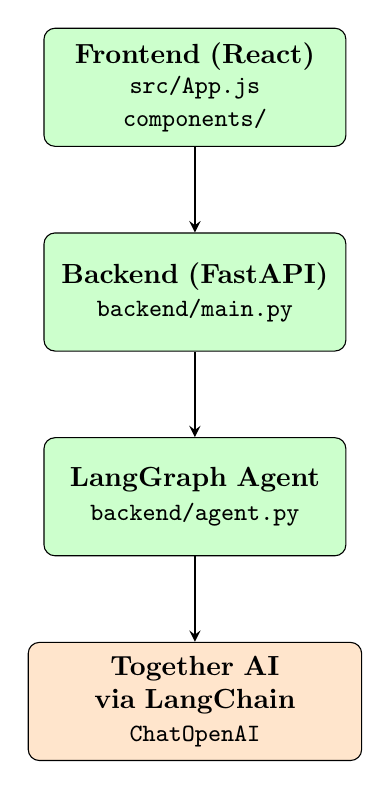
\begin{tikzpicture}[node distance=2.6cm]
            \tikzstyle{layer} = [rectangle, draw, fill=green!20, text width=3.6cm, text centered, rounded corners, minimum height=1.5cm]
            \tikzstyle{service} = [rectangle, draw, fill=orange!20, text width=4.0cm, text centered, rounded corners, minimum height=1.5cm]
            \tikzstyle{arrow} = [thick,->,>=stealth]

            \node (frontend) [layer] {\textbf{Frontend (React)}\\\small{\texttt{src/App.js}\\\texttt{components/}}};
            \node (backend) [layer, below of=frontend] {\textbf{Backend (FastAPI)}\\\small{\texttt{backend/main.py}}};
            \node (agent)   [layer, below of=backend] {\textbf{LangGraph Agent}\\\small{\texttt{backend/agent.py}}};
            \node (llm) [service, below of=agent] {\textbf{Together AI via LangChain}\\\small{\texttt{ChatOpenAI}}};

            \draw [arrow] (frontend) -- (backend);
            \draw [arrow] (backend) -- (agent);
            \draw [arrow] (agent) -- (llm);
        \end{tikzpicture}
    \end{center}
\end{frame}

%------------------------------------------------

    \begin{frame}{Agent Workflow (LangGraph)}
        \begin{center}
            \includegraphics[width=0.9\textwidth]{code_structure.png}
        \end{center}
        \vspace{0.3cm}
        \small 
        The LangGraph agent implements a three-stage workflow:
        \begin{itemize}
            \item \textbf{Stage 1}: Mode-based query optimization (tactile/vision/combined)
            \item \textbf{Stage 2}: Few-shot prompt construction with modality-specific builders
            \item \textbf{Stage 3}: Single \texttt{ChatOpenAI} call to Together AI for inference
        \end{itemize}
    \end{frame}

    \begin{frame}{Prompt Design \& Few-shot Examples}
        \begin{itemize}
            \item \textbf{Standardized Output}: comma-separated adjectives (top 5), no sentences.
            \item \textbf{Templates}: \texttt{TASK\_PROMPT\_TACTILE}, \texttt{TASK\_PROMPT\_VISION}, \texttt{TASK\_PROMPT\_COMBINED} in \texttt{backend/prompt\_templates.py}.
            \item \textbf{Few-shot}: up to 5 curated pairs from \texttt{backend/images\_rgb} and \texttt{backend/images\_tac}.
            \item \textbf{Compliance}: Combined mode sends each image in a \textit{separate} message to respect API limits.
        \end{itemize}
        \vspace{0.3cm}
        \begin{block}{Example Output}
            \small absorbent, fluffy, soft, yielding, warm
        \end{block}
    \end{frame}

    \begin{frame}{API and Data Flow}
        \textbf{Endpoint}: \texttt{POST /api/reasoning} (see \texttt{backend/main.py})
        \begin{itemize}
            \item \texttt{question} (string), \texttt{mode} in \{tactile, vision, combined\}
            \item Optional base64 images: \texttt{tactile\_image}, \texttt{vision\_image}
            \item Validation by mode; CORS enabled for React dev server
        \end{itemize}
        \vspace{0.3cm}
        \textbf{Frontend}: React components \texttt{ControlsSection.js}, \texttt{ImageUpload.js}, \texttt{ResponseSection.js}
        \begin{itemize}
            \item Collect inputs, encode images, call backend, display adjective list
        \end{itemize}
    \end{frame}

%------------------------------------------------
\section{Results}
%------------------------------------------------

\begin{frame}{Qualitative Examples (Placeholders)}
    \begin{columns}[c]
        \column{.48\textwidth}
        \textbf{Inputs}
        \begin{itemize}
            \item RGB photograph
            \item Tactile visualization
        \end{itemize}
        \vspace{0.2cm}
        \imgph{6.0cm}{3.5cm}
        \vspace{0.3cm}
        \imgph{6.0cm}{3.5cm}

        \column{.48\textwidth}
        \textbf{Model Output}
        \begin{block}{Comma-separated adjectives}
            \small rough, rigid, matte, coarse, non-absorbent
        \end{block}
        \vspace{0.2cm}
        \textbf{Notes}
        \begin{itemize}
            \item Replace placeholders with your experimental images
            \item Provide brief interpretation under each example
        \end{itemize}
    \end{columns}
\end{frame}

\begin{frame}{Quantitative Results (Placeholder)}
    \textbf{Planned metrics}
    \begin{itemize}
        \item Top-$k$ match rate for ground-truth adjective sets
        \item Agreement vs. human labels on curated test set
        \item Modality ablation: vision-only vs. tactile-only vs. combined
    \end{itemize}
    \vspace{0.4cm}
    \begin{center}
        \imgph{11.5cm}{5.0cm}
    \end{center}
\end{frame}

%------------------------------------------------
\section{Discussion and Conclusions}
%------------------------------------------------

\begin{frame}{Discussion}
    \textbf{What the results suggest}
    \begin{itemize}
        \item Standardized prompts and few-shot examples stabilize outputs across inputs
        \item Combined modality likely improves attribute coverage and specificity
    \end{itemize}
    \vspace{0.3cm}
    \textbf{Limitations}
    \begin{itemize}
        \item Limited labeled data; qualitative-heavy evaluation
        \item Sensitivity to image quality and sensor visualization style
    \end{itemize}
\end{frame}

\begin{frame}{Conclusions and Future Work}
    \textbf{Conclusions}
    \begin{itemize}
        \item Built an interactive multimodal system integrating React, FastAPI, LangGraph, and Together AI
        \item Mode-aware agent reliably produces concise tactile descriptors
    \end{itemize}
    \vspace{0.3cm}
    \textbf{Future Work}
    \begin{itemize}
        \item Collect annotated dataset and report quantitative metrics
        \item Explore retrieval-augmented prompting and better few-shot selection
        \item Add persistence, batch processing, and richer UI affordances
    \end{itemize}
\end{frame}


%------------------------------------------------
\section{Acknowledgements}
%------------------------------------------------

\begin{frame}{Acknowledgements}
    \begin{itemize}
        \item Supervisor: Dr. [Supervisor Name]
        \item Lab colleagues and friends for feedback and testing
        \item Together AI for model access and LangChain community resources
    \end{itemize}
    \vspace{0.4cm}
    \begin{center}
        {\Large \textbf{Thank You!}}\\
        \vspace{0.2cm}
        \small Questions welcome
    \end{center}
\end{frame}

%------------------------------------------------

%----------------------------------------------------------------------------------------

\end{document}